El \textit{algoritmo de Dijkstra} calcula los caminos de coste mínimo entre un \textbf{origen} y \textbf{todos los demás vértices} del grafo \(G\).

\begin{minted}[breaklines]{c++}
template <typename tCoste>
vector<tCoste>
  Dijkstra(const GrafoP<tCoste>& G, typename GrafoP<tCoste>::vertice origen, vector<typename GrafoP<tCoste>::vertice& P);
\end{minted}

Como salida tenemos:
\begin{itemize}
  \item \textbf{Vector de costes mínimos} de tamaño \verb|G.numVert()|.
  \item \textbf{Vector de vértices} (P) de tamaño \verb|G.numVert()|, tal que \verb|P[i]| es el vértice anterior a \(i\) en el camino de costes mínimo (origen, i).
\end{itemize}

\textit{NOTA:} Un grafo no dirigido, es un grafo dirigido pero con flechas en ambas direcciones, por tanto, si tenemos un algoritmo que funciona para grafos dirigidos también serán válidos para grafos no dirigidos.

\textit{NOTA:} \textbf{Dijkstra Inverso} es igual que Dijkstra pero con la diferencia que en vez de tener un origen vamos a tener un destino.

\subsection{Ejemplo algoritmo Dijkstra}
\begin{figure}[h]
  \begin{minipage}{0.5\textwidth}
    Encontramos un vector de booleanos, que indica si hemos pasado o no por dicho vértice.
  
    Estos vértices en el vector `S' se inicializan a \texttt{False} y partimos desde el origen a todos los vértices del grafo.
  \end{minipage}
  \hfill
  \begin{minipage}{0.4\textwidth}
   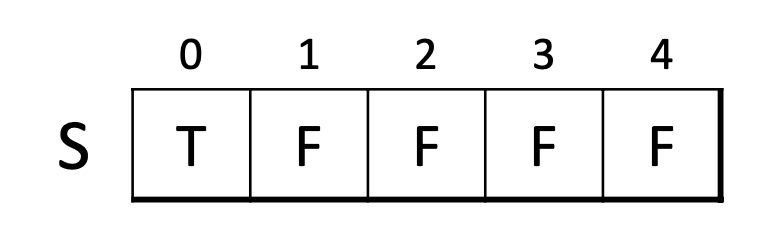
\includegraphics[width=\textwidth]{assets/dij2.png} 
  \end{minipage}
\end{figure}

El algoritmo se acaba cuando hemos pasado por todos los vétices del grafo, es decir, el vector de booleano está lleno con valores \texttt{True}.

Como hemos comentado previamente, el algoritmo devuelve dos cosas: el vector de vértices `camino' y el coste mínimo `distancia'.
\newpage
\begin{figure}[h]
  \begin{minipage}{0.4\textwidth}
    \begin{center}
      \textbf{Distancia}
      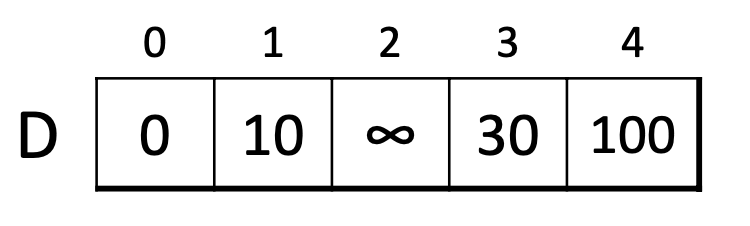
\includegraphics[width=\textwidth]{assets/dij3.png}
    \end{center}
  Es el \textbf{coste mínimo} de ir desde el origen hasta cualquier otro vértice del grafo.

  En este algoritmo siempre partimos del vértice origen.

  Hacemos uso de un vector y este se inicializa con los costes directos entre el origen y los demás vértices del grafo.

  \end{minipage}
  \hfill
  \begin{minipage}{0.4\textwidth}
  \vspace*{-2cm}
  \begin{center}
    \textbf{Camino}
    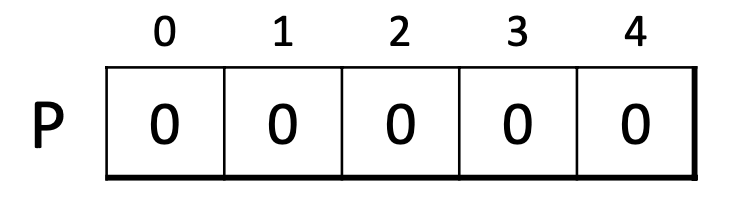
\includegraphics[width=\textwidth]{assets/dij4.png} 
  \end{center}
  Es un \textbf{vector de vértices}, cuando el camino es directo se inicializa a `0'.

  Nos permite recuperar el camino, que son los vértices desde el origen hasta el destino por los que ha pasado.
  \end{minipage}
\end{figure}

Gracias a este algoritmo vamos a poder reducir el coste de ir de un vértice a otro, calculando los costes de ir de un vértice a otro y quedándonos con el mínimo.

Tenemos el grafo y la matriz de costes siguientes:

\begin{figure}[h]
  \begin{center}
    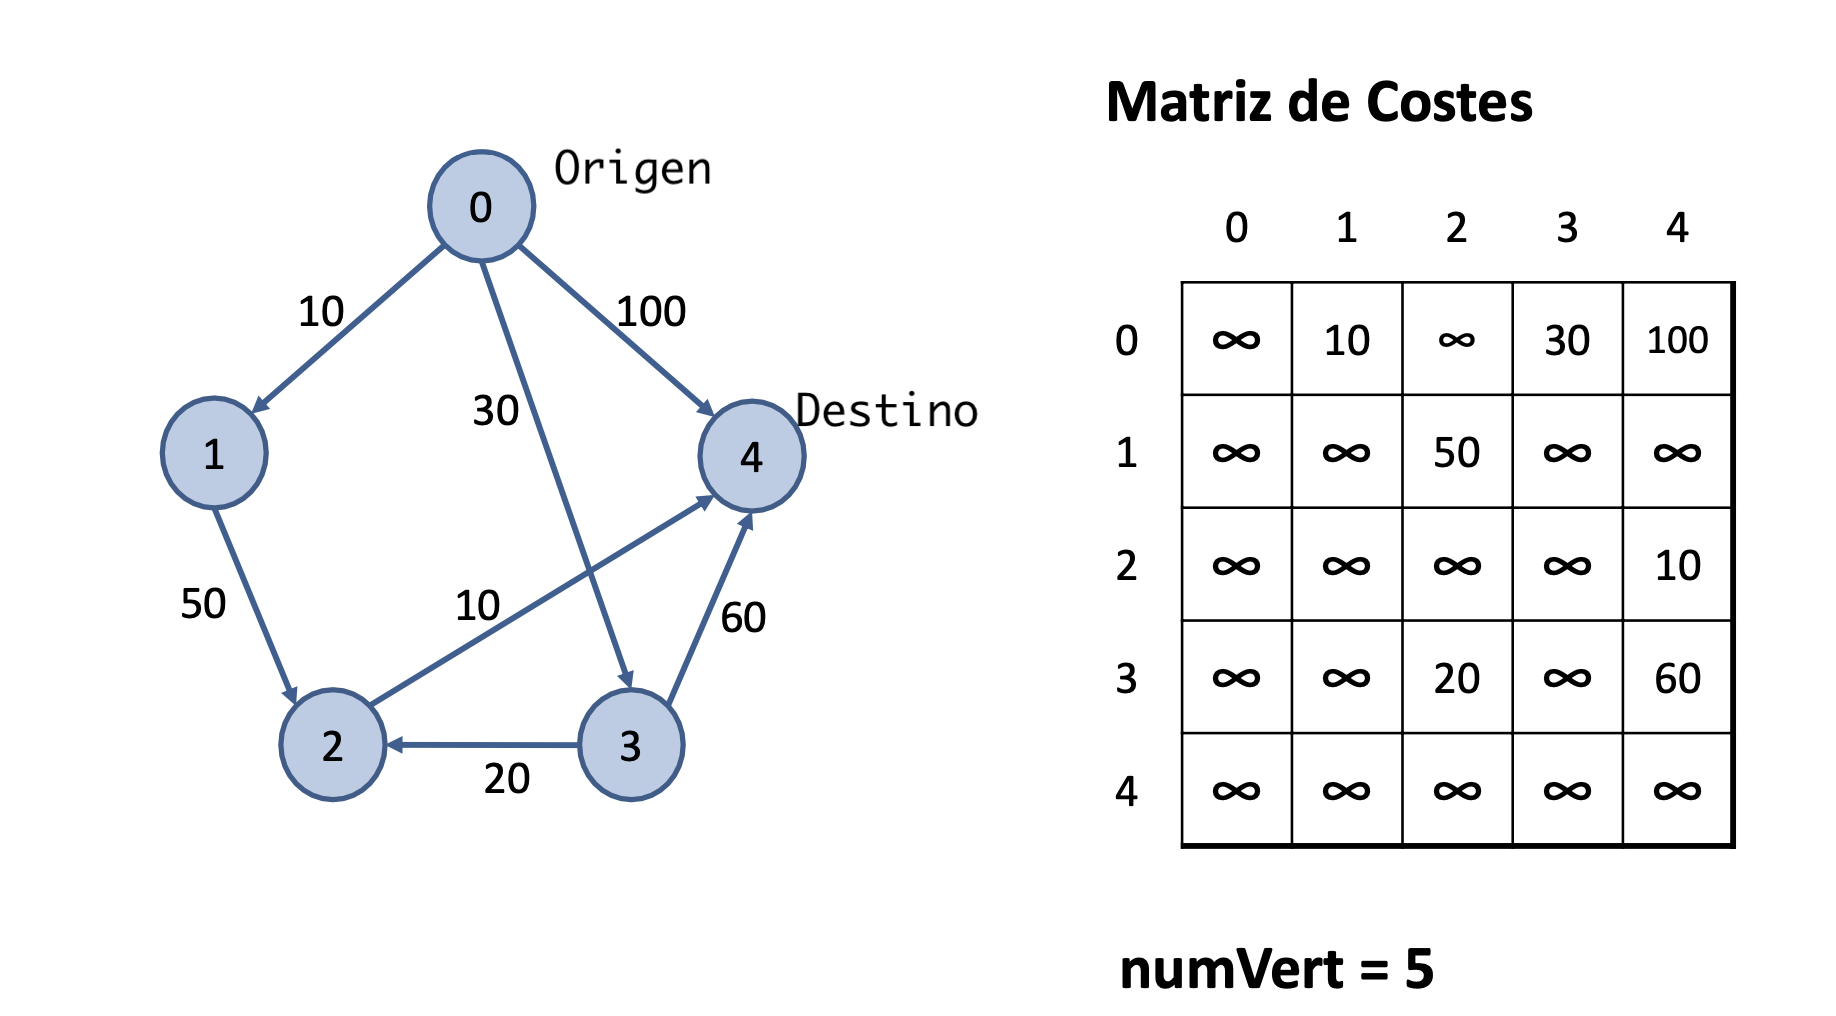
\includegraphics[width=0.7\textwidth]{assets/dij1.png}
  \end{center}
\end{figure}


Vemos que tenemos el grafo anterior y queremos ir desde el vértice 0 `origen' hasta el vértice 4 `destino'.

Para ello, en el vector de costes mínimos `D' tenemos los valores obtenidos previamente arriba, pero vamos a realizar una optimización del mismo y además encontramos el vector de vértices `P', que está inicializado a 0 (hay camino directo) ó \textit{infinito} (no hay camino directo).

Los vectores comentados anteriormente ya tienen almacenado tanto los costes como los vértices por donde pasan, pero no siempre es eficiente hacer uso de los caminos directos, por eso vamos a realiar un par de modificaciones.

Vemos que no hay camino directo entre el origen y el vértice `2', por tanto, para acceder a él lo haremos desde el vértice `1' y su coste será el de ir desde origen a `1' \((0\rightarrow1)\) más el de `1' a `2'(\(1\rightarrow2\)), además en el vector de vértices en la `casilla' del número `2' pondremos `1' (vértice que accede a él) y en el vector de booleanos podemos que ya se ha pasado por el vértice `0'(origen) y `1'.
\begin{center}
  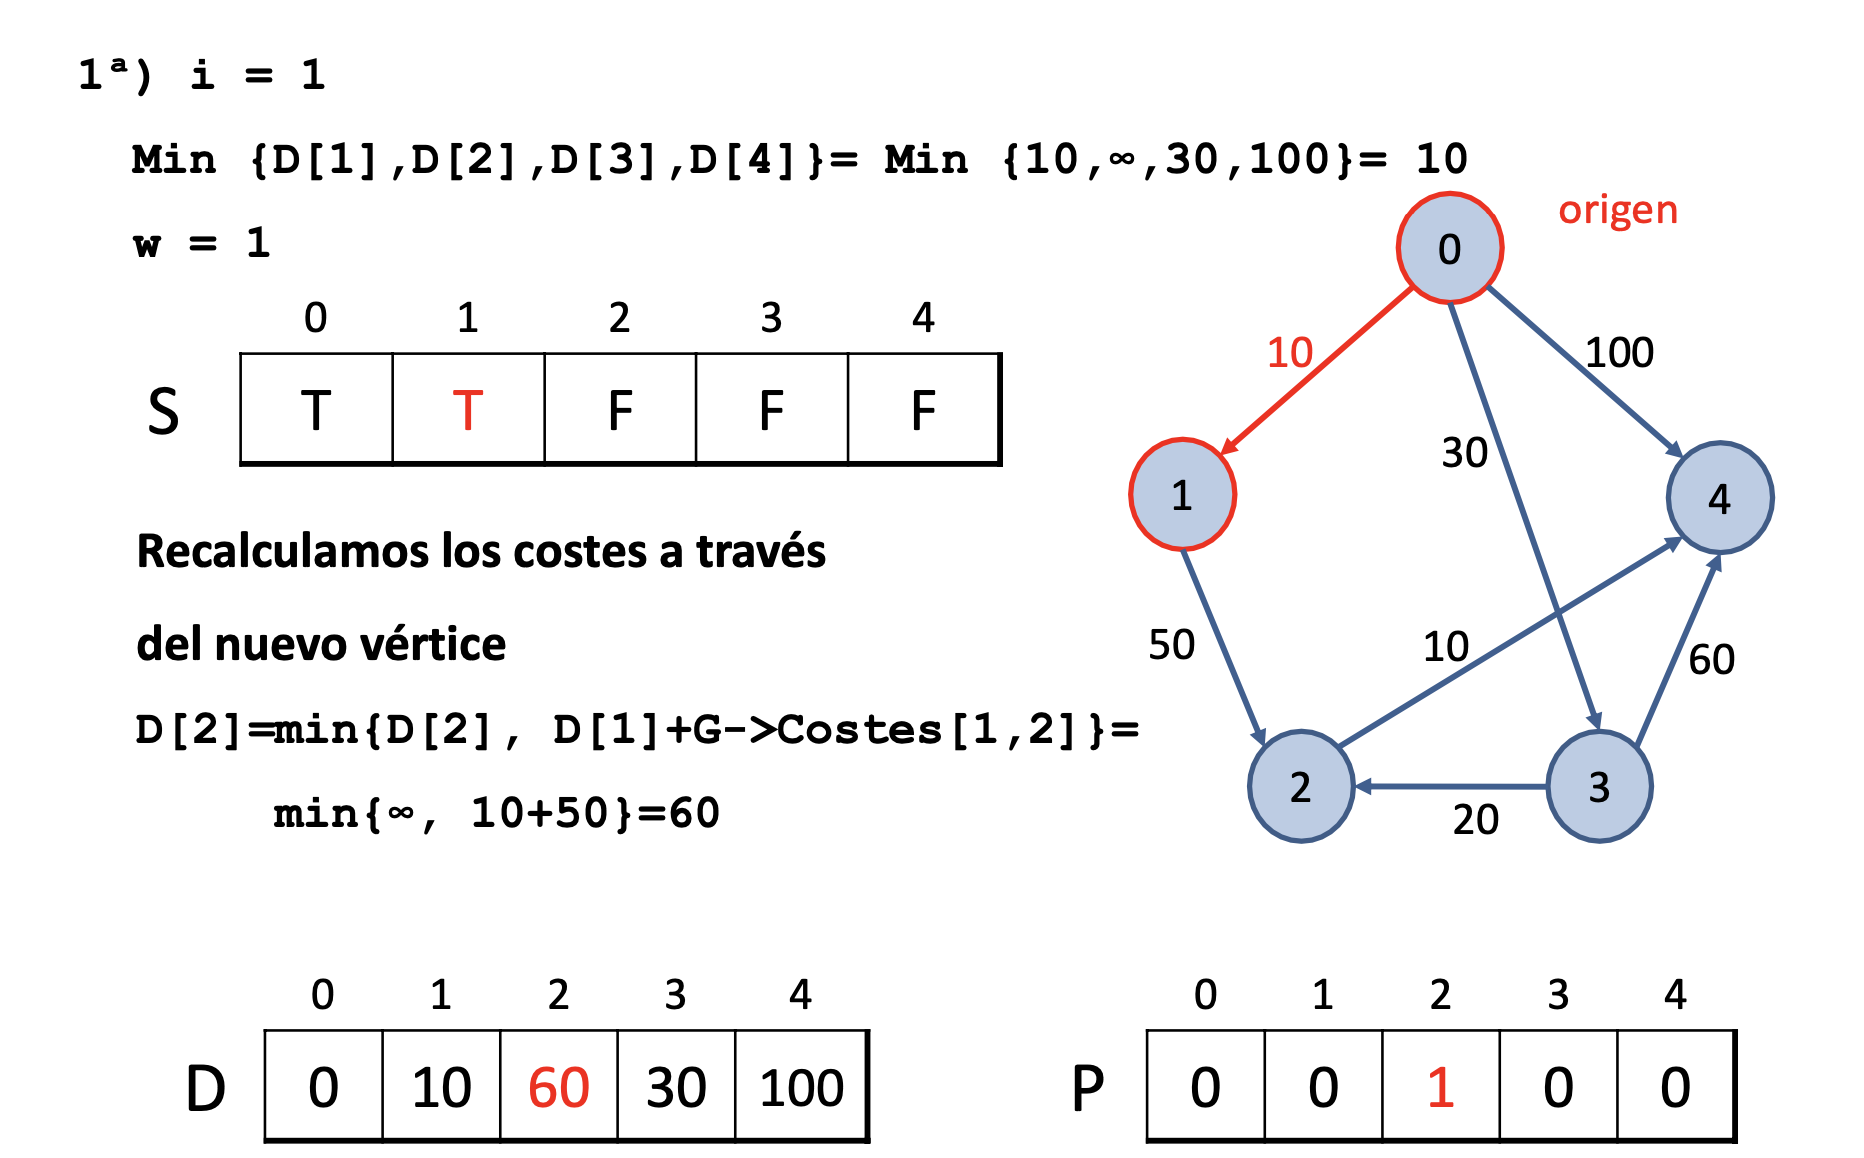
\includegraphics[width=0.7\textwidth]{assets/dij5.png}
\end{center}

El coste de ir al vértice `3'(\(0\rightarrow3\)) seguirá siendo el mismo, ya que es el único camino que hay y este es de coste 30, se dejan igual los vectores tanto de coste como de vértices y se indica en el vector de booleanos que ya hemos pasado por el vértice `3'.

\begin{figure}[h]
  \begin{center}
    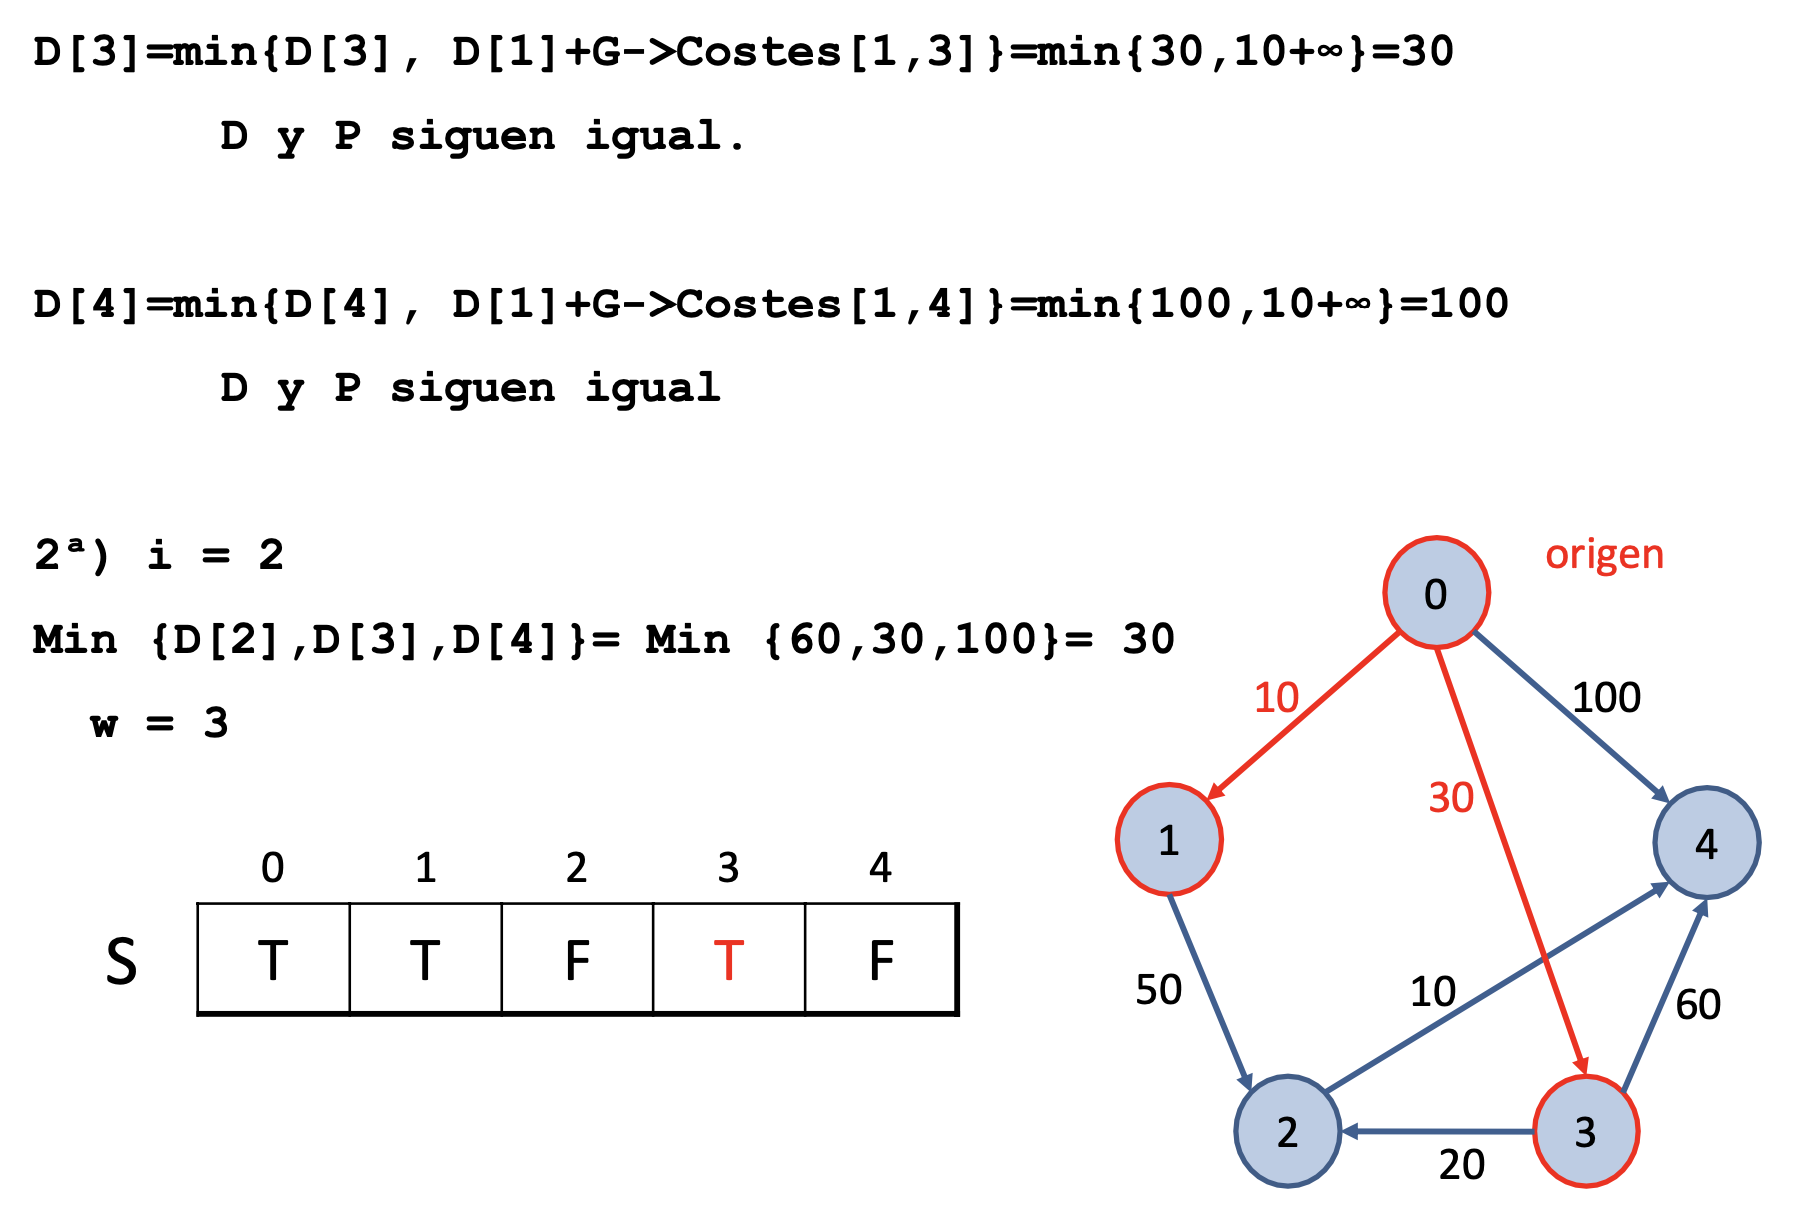
\includegraphics[width=0.7\textwidth]{assets/dij6.png}
  \end{center}
\end{figure}

Ahora nos queda calcular el coste de ir desde el origen al vértice `4', para ello tenemos 4 maneras:
\begin{itemize}
  \item camino directo: (\(0\rightarrow4\)) con un coste de 100.
  \item camino secundario: (\(0\rightarrow1\rightarrow2\rightarrow4\)) con un coste de 70.
  \item camino secundario: (\(0\rightarrow3\rightarrow2\rightarrow4\)) con un coste de 60.
  \item camino secundario: (\(0\rightarrow3\rightarrow4\)) con un coste de 90.
\end{itemize}

Como queremos obtener el coste mínimo, nos vamos a quedar con el camino cuyo coste sea el más pequeño, en este caso será el camino secundario (\(0\rightarrow3\rightarrow2\rightarrow4\)) que tiene un coste de 60.

Finalmente, actualizamos los vectores de costes, de vértices y el de booleanos el cual tendría que tener a \texttt{True} todos los vértices del grafo.
\newpage
\underbar{\large\textbf{Resultado:}}
\begin{figure}[h]
  \begin{center}
    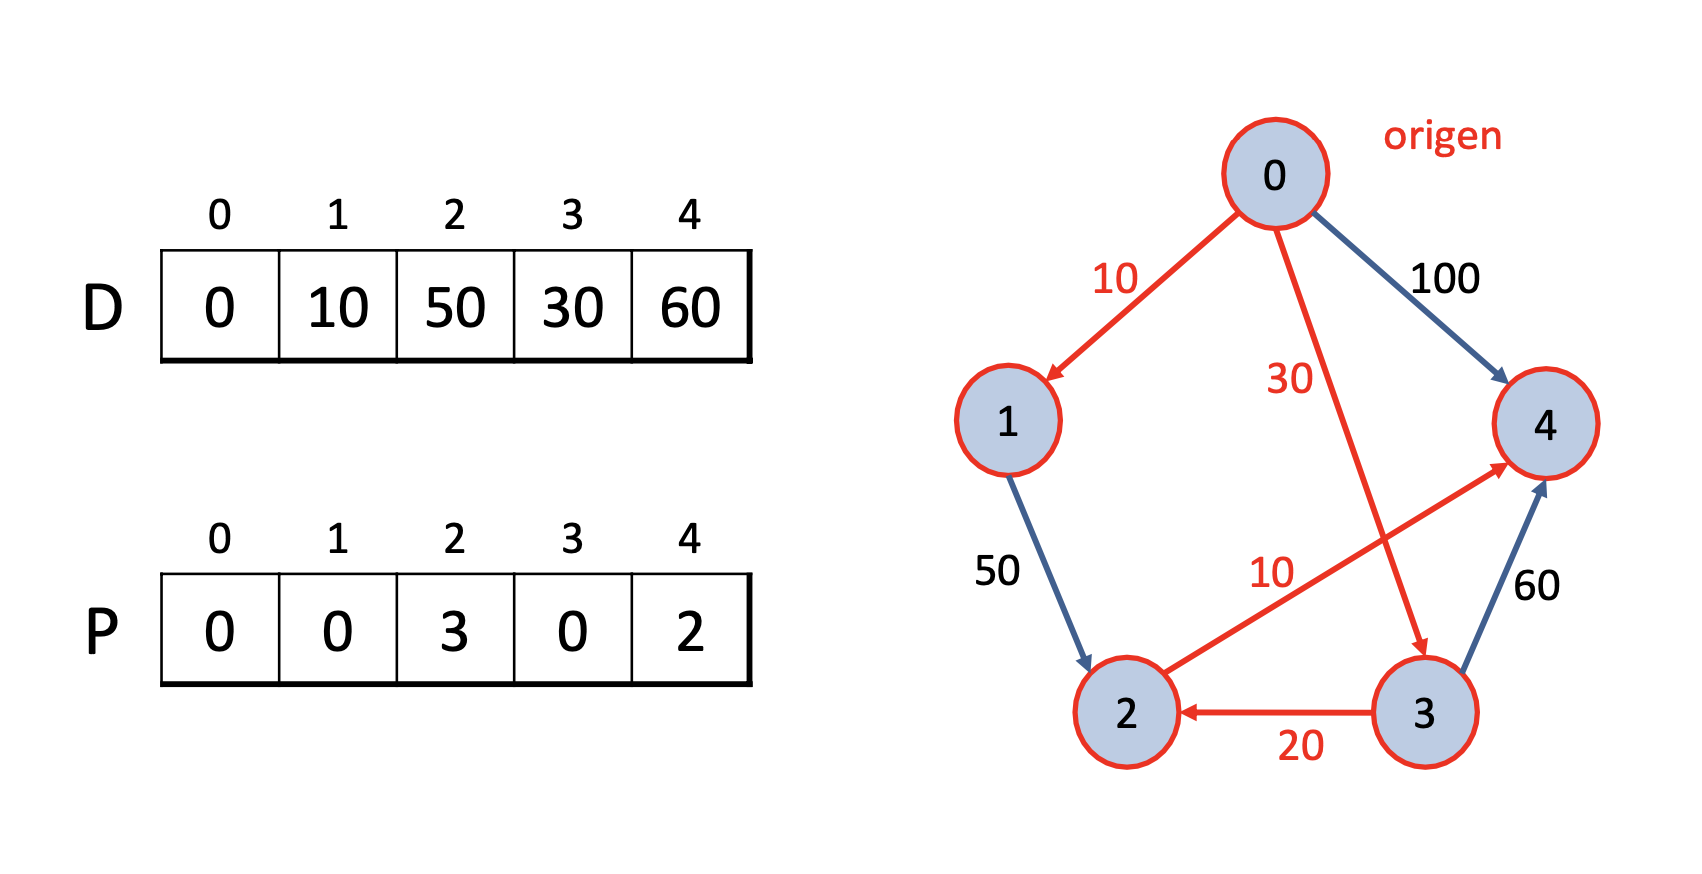
\includegraphics[width=0.7\textwidth]{assets/dij8.png}
  \end{center}
  \caption{Resultado de aplicar Dijkstra}
\end{figure}
\subsection{Código del algoritmo Dijkstra}
\subsubsection*{Suma de costes}
Como hemos comentado anteriormente haremos uso de un tipo de dato llamado \texttt{INFINITO} para indicar que no hay camino directo entre dos vértices del grafo.
\begin{minted}[breaklines]{C++}
template <typename tCoste> tCoste suma(tCoste x, tCoste y){
  //vamos a crear un alias para el tipo de dato infinito
  const tCoste INFINITO = GrafoP<tCoste>::INFINITO;
  if(x == INFINITO || y == INFINITO) return INFINITO;
  else return x+y;
}
\end{minted}

\subsubsection*{Algoritmo Dijkstra}
\begin{minted}[breaklines]{C++}
template <typename tCoste> vector<tCoste> Dijkstra (const GrafoP<tCoste>& G,typename GrafoP<tCoste>::vertice origen, vector<typename GrafoP<tCoste>::vertice>& vertice){
  typedef typename GrafoP<tCoste>::vertice vertice;
  vertice v,w;
  const size_t n = G.numVert(); //guardamos el numero de vertices
  vector<bool> S(n,false); //vector de booleanos inicializado a falso
  vector<tCoste> D; //Costes minimos
  //Inicializamos D y P con los caminos directos desde el origen
  D = G[origen];
  D[origen] = 0;
  P = vector<vertice>(n,origen);
  S[origen] = true;
  // Localizar vértice w no incluido en S con menor coste desde origen.
  for(size_t i = 1; i<=n-2; i++){
    tCoste costeMinimo = GrafoP<tCoste>::INFINITO;
    for(v=0;v<= n-1; v++){
      if(!S[v] && D[V] <=costeMinimo){
        costeMinimo = D[v];
        w = v;
      }
    S[w] = true;
  //Recalcular coste hasta cada v no incluido en S, a través de w.
  //Aqui optimizamos de verdad, donde se recálcala los valores del vector.
  for(v=0; v<=n-1; v++)
    if(!S[v]){
      tCoste Owv = suma(D[w], G[w][v]);
      if(Owv < D[v]){
        D[v] = Owv; //Coste de ir del origen a v a través de w.
        P[v] = w;
      }
    }
  }
  return D;
}
\end{minted}
\subsubsection*{Método Camino}
Este método recibe el vértice origen, un vertice cualquiera (destino) y el vector de vértices y devuelve el camino.

\begin{minted}[breaklines]{C++}
template <typename tCoste> typename GrafoP<tCoste>::tCamino camino(typename GrafoP<tCoste>::vertice orig, typename GrafoP<tCoste>::vertice v,const vector<typename GrafoP<tCoste>::vertice>& P){
  typename GrafoP<tCoste>::tCamino C;
  C.insertar(v,C.primera());
  do{
    C.insertar(P[v], C.primera());
    v = P[v];
  }while(v!=orig);
  return C;
}
\end{minted}
